%%%%%%%%%%%%%%%%%%%%%%%%%%%%%%%%%%%%%%%%%%%%%%%%%%%
%% P3: Phenomenology of Particle Physics                         
%%
%% Author:  André Rubbia                   		 
%%
%% Figure 14.4 Schematic of the $g-2$ muon storage ring experiment.
%%
%% This work is licensed under the Creative Commons Attribution 4.0 International License. 
%% To view a copy of this license, visit http://creativecommons.org/licenses/by/4.0/ or 
%% send a letter to Creative Commons, PO Box 1866, Mountain View, CA 94042, USA.
%%
%%%%%%%%%%%%%%%%%%%%%%%%%%%%%%%%%%%%%%%%%%%%%%%%%%%

\documentclass[a4paper,10pt]{article}

\usepackage[T1]{fontenc}
\usepackage[utf8]{inputenc}
\usepackage{lmodern}
\usepackage[labelfont=bf]{caption}
\usepackage{upgreek}

\usepackage{tikz}
\usepackage{pgfplots}
\pgfplotsset{compat=1.17}
\usepgfplotslibrary{ternary}
\usepgfplotslibrary{fillbetween}
\usepgfplotslibrary{external}

\usepackage{braket}

\def\d{\mathrm{d}}

\pgfkeys{/pgf/number format/.cd,1000 sep={}}

\begin{document}

%%%%%%%%%%%%%%%%% FIGURE %%%%%%%%%%%%%%%%%%%%%%%%%%%%%%%%%%
\begin{figure}[htb]
\begin{center}
    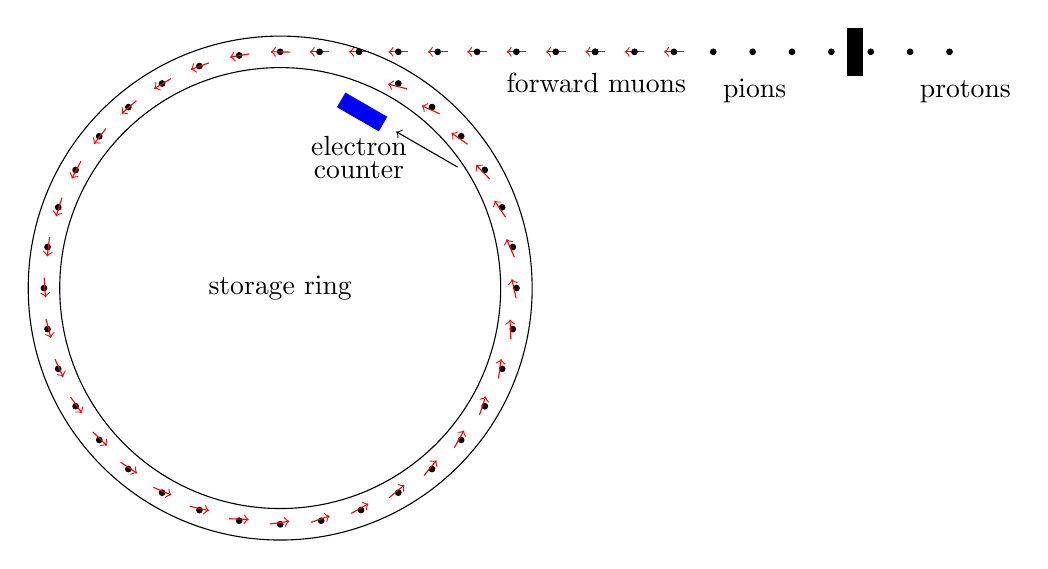
\begin{tikzpicture}[scale=1]
         \foreach \x in {0,...,9}
	        	\draw[red,->] (\x/2+0.5+0.125, 3) -- +(-0.25,0);
         \foreach \x in {0,...,7}
         	\draw[fill] (\x/2+0.5, 3) circle (1pt);
         \foreach \x in {9,...,42}
         	\draw[fill] ({3*cos(\x*10)},{3*sin(\x*10)}) circle (1pt);
         \foreach \x in {0,...,33}
         	\draw[red,->] ({3*cos((\x+8.75)*10)},{3*sin((\x+8.75)*10)}) -- +({-0.25*sin((\x+8.5)*10.5)},{0.25*cos((\x+8.5)*10.5)});
        	\draw (0,0) circle (3.2cm);
        	\draw (0,0) circle (2.8cm);
         \foreach \x in {0,...,9}
	         \draw[fill] (\x/2+4, 3) circle (1pt);
 	\draw[fill, color=black] (7.2,2.7) rectangle +(0.2,0.6);
	 \node[right] at (8,2.5) {protons};
	 \node[right] at (5.5,2.5) {pions};
	 \node[right] at (2.75,2.6) {forward muons};
	 \begin{scope}[shift={(1.25,2)}, rotate=60]
	 	\draw[fill, color=blue] (0,0) rectangle +(0.2,0.6);
		\draw[<-] (0.1,-0.2) -- (0.1,-1.1);
	 \end{scope}
	 \node[] at (1.,1.8) {electron};
	 \node[] at (1.,1.5) {counter};
	 \node[] at (0,0) {storage ring};
     \end{tikzpicture}
\caption{Schematic of the $g-2$ muon storage ring experiment. High-energy protons hit a target,
producing secondary pions. These latter shortly decay into muons (and neutrinos). The muons are
polarized. The arrows symbolize the
muon spin direction. Muons of a given momentum are trapped in the storage ring until they decay. The
decay electron is analyzed to determine the muon polarization. At every turn, the angle between the momentum
and the spin of the muon increases due to the anomalous $g-2$ term, as schematically illustrated.}
\end{center}
\end{figure}
%%%%%%%%%%%%%%%%% END FIGURE %%%%%%%%%%%%%%%%%%%%%%%%%%%%%%
%

\end{document}
